\chapter{插值法}

\section{引言}

\begin{definition}[插值法]
    设函数$y=f(x)$在区间$[a,b]$上有定义, 且已知在点$a\le x_0\le x_1<\cdots<x_n\le b$上的值$y_0,y_1,\cdots,y_n$, 若存在
    一简单函数$P(x)$, 使
    \begin{equation}\label{eqn:2.1.1}
        P(x_i) = y_i,i=0,1,\cdots,n
    \end{equation}
    成立, 则称$P(x)$为函数$f(x)$的\emph{插值函数}, 点$x_0,x_1,\cdots,x_n$为\emph{插值节点}, 包括插值节点的区间$[a,b]$称为
    \emph{插值区间}, 求插值函数$P(x)$的方法称为\emph{插值法}.
\end{definition}

\begin{definition}[多项式插值]
    若$P(x)$是次数不超过$n$的代数多项式, 即
    \begin{equation}\label{eqn:2.1.2}
        P(x) = a_0+a_1x+\cdots+a_nx^n
    \end{equation}
    其中$a_i$为实数, 则称$P(x)$为\emph{插值多项式}, 相应的插值法称为\emph{多项式插值}.
\end{definition}

本章所讨论的主要内容是\emph{多项式插值}.

在寻找插值多项式之前, 需要对其存在性与唯一性进行讨论\footnote{存在性表明插值多项式存在, 唯一性表明无论采用哪种插值方法,
得到的结果是唯一的.}. 给出如下定理:

\begin{theorem}
    对于给定互异节点$x_0,x_1,\cdots,x_n$, 满足插值条件式(\ref{eqn:2.1.1})的$n$阶插值多项式(\ref{eqn:2.1.2})存在且唯一.
\end{theorem}

\begin{proof}
    设所要构造的插值多项式为
    \begin{equation*}
        P_n(x)=a_0+a_1x+\cdots+a_nx^n
    \end{equation*}
    由插值条件
    \begin{equation*}
        P_n(x_i) = y_i, i=0,1,\cdots,n
    \end{equation*}
    得如下线性方程组
    \begin{equation*}
        \begin{cases}
            1\cdot a_0+x_0a_1+\cdots+x_0^na_n=y_0\\
            1\cdot a_0+x_1a_1+\cdots+x_1^na_n=y_1\\
            \vdots\\
            1\cdot a_0+x_na_1+\cdots+x_n^na_n=y_n
        \end{cases}
    \end{equation*}
    求解$a_0, a_1, \cdots, a_n$, 计算系数行列式
    \begin{equation*}
        D = \mqty|1&x_0&x_0^2&\cdots&x_0^n\\
        1&x_1&x_1^2&\cdots&x_1^n\\
        \vdots&\vdots&\vdots&&\vdots\\
        1&x_n&x_n^2&\cdots&x_n^n|
    \end{equation*}
    该行列式为Vandermonde行列式, 其值为
    \begin{equation*}
        D = \prod_{0\le j<i\le n}(x_i-x_j)
    \end{equation*}
    当$x_i\ne x_j$时, $D\ne 0$, 即$P_n(x)$由$a_0, a_1, \cdots, a_n$唯一确定
\end{proof}

在实际计算过程中, 直接求解方程组往往计算量较大, 且方程组可能具有\emph{病态性}. 例如, 对于$x_1,x_2,x_3,x_4$, 若值分别为
0.1, 0.2, 0.3, 0.4, 则行列式$D = 1.2\times10^{-6}\approx0$.

因此, 通常的做法是在$n$次多项式空间中寻找一组基函数
\begin{equation*}
    \varphi_0(x),\varphi_1(x),\cdots,\varphi_n(x)
\end{equation*}
使得
\begin{equation*}
    P_n(x)=a_0\varphi_0(x)+a_1\varphi_1(x)\cdots+a_n\varphi_n(x)
\end{equation*}
不同的基函数对应不同的插值法. 本章重点讨论Lagrange插值法与Newton插值法.

\section{Lagrange插值法}

\subsection{线性插值}

\begin{example}
    对于节点$(x_0,y_0),(x_1,y_1)$, 求一次多项式
\end{example}

\begin{solution}
    利用直线的两点式, 不难得到其插值多项式为
    \begin{align*}
        P_1 &= \left(\frac{x-x_1}{x_0-x_1}\right)y_0+\left(\frac{x-x_0}{x_1-x_0}\right)y_1\\
        &=l_0(x)y_0+l_1(x)y_1=\sum_{i=0}^1l_i(x)y_i
    \end{align*}
\end{solution}

在这里, 称
\begin{equation*}
    l_0(x)=\frac{x-x_0}{x_0-x_1}, l_1(x) = \frac{x-x_0}{x_1-x_0}
\end{equation*}
为一次Lagrange插值基函数.

不难验证, 对于一次Lagrange插值基函数而言, 存在如下性质
\begin{itemize}
    \item $l_0(x), l_1(x)$均为一次多项式
    \item $l_0(x_0)=1, l_1(x_0)=0, l_0(x_1)=0, l_1(x_1)=1$
\end{itemize}

\subsection{抛物插值}

与线性插值类似, 对于抛物插值, 设有三个插值点$(x_0,y_0),(x_1,y_1),(x_2,y_2)$, 可得其插值多项式为

\begin{equation*}
    P_2(x)=y_0l_0(x)+y_1l_1(x)+y_2l_2(x)
\end{equation*}
其中$l_0(x),l_1(x),l_2(x)$均为二次多项式, 且有
\begin{align*}
    l_0(x_0)=1,l_1(x_0)=0,l_2(x_0)=0\\
    l_0(x_1)=0,l_1(x_1)=1,l_2(x_1)=0\\
    l_0(x_2)=0,l_1(x_2)=0,l_2(x_2)=1
\end{align*}

\subsection{Lagrange插值多项式}

将上述结论推广至$n$阶情况.即假设有$n+1$个节点$x_0,x_1,\cdots,x_n$的$n$阶插值多项式$L_n(x)$, 且满足条件
\begin{equation*}
    L_n(x_i) = y_i,i=1,2,\cdots,n
\end{equation*}

类似于线性插值和抛物插值, 我们首先需要定义出\emph{基函数}.

\begin{definition}
    若$n$次多项式$l_j(x),j=0,1,\cdots,n$在$n+1$个节点$x_0<x_1<\cdots<x_n$上满足条件
    \begin{equation*}
        l_j(x_k)=\begin{cases}
            1,k=j\\
            0,k\ne j
        \end{cases},j,k=0,1,\cdots,n
    \end{equation*}
    则称这$n+1$个$n$次多项式$l_0(x),l_1(x),\cdots,l_n(x)$为节点$x_0,x_1,\cdots,x_n$上的$n$次插值基函数.
\end{definition}

利用其性质, 可以得到基函数形式为
\begin{equation*}
    l_k(x)=\frac{(x-x_0)\cdots(x-x_{k-1})(x-x_{k+1})\cdots(x-x_n)}{(x_k-x_0)\cdots(x_k-x_{k-1})
    (x_k-x_{k+1})\cdots(x_k-x_n)}, k=0,1,\cdots,n
\end{equation*}

\begin{extend}
    下面将说明如何计算基函数的形式.

    利用性质, 可知对于$l_k(x),k=0,1,\cdots,n$, 当$x\ne x_k$时, 其函数值为0. 则可以将其分解为若干因
    式$(x-x_j),j=0,1,\cdots,n$且$j\ne k$, 即
    \begin{equation*}
        l_k(x)=\lambda(x-x_0)(x-x_1)\cdots(x-x_{k-1})(x-x_{k+1})\cdots(x-x_n),k=0,1,\cdots,n
    \end{equation*}
    
    同时, 由于当$x=x_k$时, $l_k(x_k)=1$, 可得待定系数$\lambda$为
    \begin{equation*}
        \lambda = \frac{1}{(x_k-x_0)(x_k-x_1)\cdots(x_k-x_{k-1})(x_k-x_{k+1})\cdots(x_k-x_n)},k=0,1,\cdots,n
    \end{equation*}
    代入并整理, 可得基函数的具体形式为
    \begin{equation*}
        l_k(x)=\frac{(x-x_0)\cdots(x-x_{k-1})(x-x_{k+1})\cdots(x-x_n)}{(x_k-x_0)\cdots(x_k-x_{k-1})
        (x_k-x_{k+1})\cdots(x_k-x_n)}, k=0,1,\cdots,n
    \end{equation*}
    上式因此得证.
\end{extend}

下面将试着给出基于Lagrange多项式插值的一个程序代码, 仅供参考.

\begin{lstlisting}
# 使用拉格朗日多项式插值法的实例 Exercise2-1.py
# 假设四个插值点分别为(1,2),(2,3),(3,6),(4,7)
# 实际运行时这些数据可以自行修改, 从而观察插值的实际作用.

import numpy as np
import matplotlib.pyplot as plt

def lagrange_interpolation(x, points):
    n = len(points)
    result = 0.0
    for i in range(n):
        xi, yi = points[i]
        term = yi
        for j in range(n):
            if i != j:
                xj, yj = points[j]
                term *= (x - xj) / (xi - xj)
        result += term
    return result

x = [1,2,3,4]
y = [2,3,6,7]
plt.scatter(x,y,color="red")
points = list(zip(x,y))
x = np.arange(1,5,0.01)
result = lagrange_interpolation(x, points)
plt.plot(x,result)
plt.show()
\end{lstlisting}

使用这段代码运行的结果如图\ref{fig:Lagrange多项式插值}所示.

\begin{figure}[h]
    \centering
    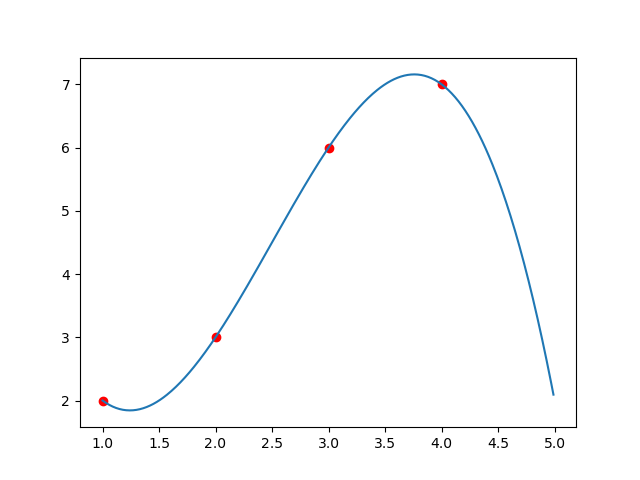
\includegraphics[width=1\linewidth]{Chapter2/graph/python/Figure2-1.png}
    \caption{Lagrange多项式插值(使用上述代码生成)}
    \label{fig:Lagrange多项式插值}
\end{figure}